\documentclass[journal]{IEEEtran}
%\IEEEoverridecommandlockouts
% The preceding line is only needed to identify funding in the first footnote. If that is unneeded, please comment it out.

% listings package for code blocks
\usepackage{listings}
\usepackage{xcolor}
\usepackage{cite}
\usepackage{verbatim}
\usepackage{graphicx}
\usepackage{parskip}

\begin{document}

% overfull \hbox .. too wide 
\setlength{\emergencystretch}{12pt}
%\setlength{\parskip}{0pt} % 1ex plus 0.5ex minus 0.2ex}
\setlength{\parindent}{10pt}

\definecolor{codegreen}{rgb}{0,0.6,0}
\definecolor{codegray}{rgb}{0.5,0.5,0.5}
\definecolor{codepurple}{rgb}{0.58,0,0.82}
\definecolor{backcolour}{rgb}{0.95,0.95,0.92}

\lstdefinestyle{mystyle}{
    backgroundcolor=\color{backcolour},   
    commentstyle=\color{codegreen},
    keywordstyle=\color{magenta},
    numberstyle=\tiny\color{codegray},
    stringstyle=\color{codepurple},
    basicstyle=\ttfamily,
    breakatwhitespace=false,         
    breaklines=true,      
    postbreak=\mbox{\textcolor{red}{$\hookrightarrow$}\space},           
    captionpos=b,
}

\lstset{style=mystyle}

\title{Developing Classification Models to Predict Diabetes}

\author{
\IEEEauthorblockN{Lillian Mueller}
\IEEEauthorblockA{lmuelle1@umd.edu}
}

\maketitle

\begin{abstract}
\label{log:abstract}
Understanding the role predictive modeling could have in the realm of diabetes prevention and maintenance holds immense potential in advancing personalized healthcare and facilitating early intervention. Leveraging a dataset consisting of diverse health indicators sourced from Kaggle, the efficacy of multiple models in identifying individuals at risk was investigated. This study examines various classification models including decision tree, logistic regression, k-nearest neighbor, naive Bayes classifier, and linear discriminant analysis. Overall, the Gaussian naive Bayes classification model exhibited the highest precision, emphasizing its capability in identifying individuals with prediabetes. However, the dataset's imbalance significantly impacted the model's overall accuracy, underscoring the need to address this issue. Insights into the comparative effectiveness of classification models for diabetes prediction can be expanded to other preventable condition given specific health indicators. 
\end{abstract}

\section{Introduction}
Diabetes is a prevalent metabolic condition that affect millions of people globally. In the United States, diabetes is the eighth leading cause of death \cite{b1}. The breadth of these conditions propels research to develop predictive methods to enable timely intervention and management. Understanding these conditions and building the capacity to predict them has great potential to improve individual health outcomes and societal outlook.

Characterized by elevated blood sugar levels, diabetes encompasses type 1, type 2, and gestational diabetes. Type 1 diabetes occurs when the body is unable to make insulin, which is a hormone that regulates glucose levels in the blood. Type 2 diabetes is the most common form of diabetes; an individual with this type cannot properly utilize insulin. Gestational diabetes can occur during pregnancy but increases the mother's chance of getting type 2 diabetes later in life \cite{b1}. Type 2 is the most common and can develop at any age, it can also be prevented. Prediabetes is a stepping stone that could be used as an indicator to being at risk of type 2 diabetes. Having prediabetes means your blood glucose levels are higher than normal \cite{b1}. Being able to identify this condition is crucial for intervention strategies such as lifestyle modifications in the form of weight loss and exercise \cite{b2}. 

This investigation explored the predictive capabilities of various classification models in determining the likelihood of an individual having diabetes, prediabetes, or no diabetes at all. The models under scrutiny include the decision tree, logistic regression, k-nearest neighbor (KNN), naïve Bayes classifier, and linear discriminant analysis (LDA). Each model offers unique methodologies and algorithms that may exhibit varying efficacy in predicting diabetes or prediabetes based on health indicators.

The investigation utilizes a comprehensive dataset sourced from Kaggle \cite{b3}. This dataset consists of health indicators such as demographic information, physiological measures, and lifestyle attributes. These attributes include age, body mass index (BMI), blood pressure, insulin levels, blood pressure, heart conditions, diet, exercise, and more. By examining these models against the dataset, this study seeks to provide insights into the most effective predictive framework for identifying individuals at risk or already affected by these metabolic conditions.

Section \ref{sec:methodology} describes how Python was used to clean the data, develop the models, and compare the models' performance. The final determination of the best fit model is in Section \ref{sec:results}. Section \ref{sec:discussion} contains discussion about performance evaluation and future research. 

\section{Methodology}
\label{sec:methodology}

This investigation entails using various classes from the library \lstinline{scikitlearn}. To develop the models: \lstinline{GaussianNB} class from the \lstinline{naive_bayes} module, the \lstinline{DecisionTreeClassifier} class from the \lstinline{tree} module, the \lstinline{LogisticRegression} class from the \lstinline{linear_model} module, the \lstinline{KNeighbors} function from the \lstinline{neighbors} module, and \lstinline{LinearDiscriminantAnalysis} class from the \lstinline{discriminant_analysis} module. Each was used to develop the naïve bayes classifier, decision tree model, the logistic regression model, KNN model, and the LDA respectively. To develop the confusion matrices and ROC (receiver operating charactoristics) of each model,  \lstinline{sklearn}'s \lstinline{metrics} module was used. Other Python libraries used along the way to help handle the data include \lstinline{matplotlib.pyplot}, \lstinline{pandas}, and \lstinline{numpy}. 

\subsection{Diabetes Dataset Preprocessing}

The dataset in this investigation was taken from Kaggle [3]. The data was downloaded from the website as a CSV file, which is a file type where the data is separated by commas. The \lstinline{pandas} library has methods that allows the analyst to directly read the data from a CSV file into a dataframe. Once the data was translated into the dataframe, each column was examined and cleaned to contain only numeric values and scaled. The target classification column contained the distinction of whether an individual had diabetes, prediabetes, or no diabetes. After encoding these classifications, 0 represented no diabetes, 1 represented prediabetes, and 2 represented diabetes. All other columns in the dataframe represented attributes that are used as features in the models to predict these classifications. The columns were all altered to only contain numerical values. The final values for each attribute are as follows: 

\begin{enumerate}
\item High Blood Pressure (HighBP)
	\begin{itemize}
        \item 0 = no
        \item 1 = yes
	\end{itemize}
\item High Cholesterol (HighChol)
	\begin{itemize}
        \item 0 = no
        \item 1 = yes
	\end{itemize}
\item Cholesterol Check within the past 5 years (CholCheck)
    \begin{itemize}
    \item 0 = no
    \item 1 = yes
    \end{itemize}
\item Body Mass Index (BMI)
\item Have you smoked 100 cigarettes (5 packs) over lifetime? (Smoker)
    \begin{itemize}
    \item 0 = no
    \item 1 = yes
    \end{itemize}
\item Stroke
    \begin{itemize}
    \item 0 = no
    \item 1 = yes
    \end{itemize}
\item Coronary Heart Disease or Myocardial Infarction (HeartDiseaseorAttack)
    \begin{itemize}
    \item 0 = no
    \item 1 = yes
    \end{itemize}
\item Physical Activity within past 30 days (not including job) (PhysActivity)
\begin{itemize}
    \item 0 = no
    \item 1 = yes
    \end{itemize}
\item Consumes Fruit $\geq$ 1 times a day (Fruits)
\begin{itemize}
    \item 0 = no
    \item 1 = yes
    \end{itemize}
\item  Consumes Vegetables $\geq$ 1 times a day (Veggies)
\begin{itemize}
    \item 0 = no
    \item 1 = yes
    \end{itemize}
\item  Heavy Drinker men $>$14 drinks, women $>$7 drinks (HvyAlcoholConsump) 
\begin{itemize}
    \item 0 = no
    \item 1 = yes
    \end{itemize}
\item  Health Care Coverage (AnyHealthcare)
\begin{itemize}
    \item 0 = no
    \item 1 = yes
    \end{itemize}
\item  Couldn't see doctor due to cost in past 12 months (NoDocbcCost)
\begin{itemize}
    \item 0 = no
    \item 1 = yes
    \end{itemize}
\item  General Health Rating (GenHlth)
\begin{itemize}
    \item 1 = excellent
    \item 2 = very good 
    \item 3 = good 
    \item 4 = fair 
    \item 5 = poor 
    \end{itemize}
\item  Number of Days Mental Health was poor within past 30 days (MentHlth)
\begin{itemize}
    \item 1-30
    \end{itemize}
\item  Number of days physical/mental health kept individual from usual activities (PhysHlth)
\begin{itemize}
    \item 1-30
    \end{itemize}
\item  Difficultly walking/climbing stairs (DiffWalk)
\begin{itemize}
    \item 0 = no
    \item 1 = yes
    \end{itemize}
\item  Sex 
\begin{itemize}
    \item 0 = female
    \item 1 = male
    \end{itemize}
\item  Age 
\begin{itemize}
    \item 1 = ages 18-24
    \item 2 = ages 25-29
    \item 3 = ages 30-34 
    \item 4 = ages 35-39
    \item 5 = ages 40-44
    \item 6 = ages 45-49
    \item 7 = ages 50-54
    \item 8 = ages 55-59
    \item 9 = ages 60-64
    \item 10 = ages 65-69
    \item 11 = ages 70-74
    \item 12 = ages 75-79
    \item 13 = 80 and older
    \end{itemize}
\item  Education 
\begin{itemize}
    \item 1 = never attended school, only kindergarden
    \item 2 = grades 1-8, elementary
    \item 3 = grades 9-11, some high school
    \item 4 = grade 12 or GED (high school graduate)
    \item 5 = College 1-3 years (Some college or technical school)
    \item 6 = college $\geq$4 years (college graduate)
    \item 9 = refused
    \end{itemize}
\item  Income 
\begin{itemize}
    \item 1 $\leq$ \$10,000
    \item 2 $\leq$ \$15,000
    \item 3 $\leq$ \$20,000 
    \item 4 $\leq$ \$25,000
    \item 5 $\leq$ \$35,000
    \item 6 $\leq$ \$50,000
    \item 7 $\leq$ \$75,000
    \item 8 $\geq$ \$75,000
    \end{itemize}
\end{enumerate}

Since there were 21 total features in the dataset, to decrease complexity and potentially increase accuracy of the models, attributes not directly related with the individuals' physical health and subjective attributes were omitted such as education, income, health care coverage, general health rating, and estimated number of days of poor mental/physical health. Overall, the dataset breakdown revealed that 84.2\% of the data represents no diabetes, 1.8\% of the dataset is classified as having prediabetes, and the remaining 14\% of the data has diabetes. 

After the diabetes dataset processed, it was split into a train group and test group using the \lstinline{model_selection.test_train_split()} function, with 2/3 of the data as the training group and the remainder as the testing group. For this dataset, since the classifications are not even, the test sets were stratified with respect to the diabetes classifications to attempt to split dataset with uniform proportions. Each model described in the following section was trained and tested using these training and testing data subsets. 

\subsection{Model Development}

Next, the models were developed and each model had to be tuned to the dataset. The first model to be trained was the decision tree model. To tune this model, the entropy and Gini index criterion were tested. Due to the large number of features, the decision trees were also constrained by varying maximum depths. Following the procedures outline in a previous study titled “Investigating Decision Trees”, the best fitting decision tree model was found to be utilizing the Gini index as the purity measurement and no constraints on the maximum depth of the tree \cite{b4}.

Since this is a multiclass dataset, \lstinline{SKLearn} has various solver algorithms to use in the optimization problem used in the logistic regression model. Those include Newton's method, the Stochastic average gradient (SAG), a variant of the SAG (SAGA), and finally the Limited-memory Broyden-Fletcher-Goldfarb-Shanno algorithm. For this application, only SAG and SAGA were investigated due to their ability to deal with large, multiclass datasets \cite{b5}. Both algorithms were tested with the dataset using no penalty and the l2 penalty. These penalties are further described in a previous study titled, “Iris Classification Using Logistic Regression” \cite{b6}. Upon running these variations of the logistic regression model, the model using SAGA solver without any penalties proved to have the greatest accuracy.  

To develop the k-nearest neighbor (KNN) model, multiple parameters were tested to tune the model to the diabetes dataset. These parameters included modifying the number of neighbors, the distance metrics used to determine similarity, and simply testing the model using uniform weights. The distance metrics in question were Euclidean, Manhattan, and cosine. Procedures to develop these methods are defined in “Evaluating the Performance of K-Nearest Neighbors Classification” \cite{b7}. The optimal parameters proved to be k = 25 using the Euclidean distance metric.

For this dataset, two versions of the naïve bayes classifier could be a fit: the Gaussian naïve Bayes and the Bernoulli naïve Bayes. The Gaussian version assumes the feature values follows a Gaussian distribution whereas the Bernoulli naïve Bayes can be used when the features are boolean vectors \cite{b8}. The Gaussian naïve Bayes classifier is run using the procedure in the previous study,  “Comparing Classifications Models Against the Naive Bayes Classifier and Linear Discriminant Analysis Model” \cite{b9}. To develop the Bernoulli model, the \lstinline{naive_bayes.BernoulliNB()} class was used.

Finally, the linear discriminant analysis (LDA) was developed using the methodology described in a previous study \cite{b9}. For this application, the default solver, the singular value decomposition, was used due to its ability to handle large numbers of features. 

\subsection{Classification Model Evaluation and Comparison}

After determining the best version of each model for the diabetes dataset, they were evaluated based on performance and compared. To start, a confusion matrix was created for each model to better visualize how each model performed. The process by which to develop the confusion matrices and its visualization is described in “Evaluating Classifications Models using Confusion Matrices” \cite{b10}. These matrices enable the analyst to visually evaluate the models' performance and derive trade-offs between true positives and false positives for each individual classification.  

To compare and rank the models, a ROC curve was created for each model to find the models AUC (area under the curve). This value is a scalar value that allows the user to evaluate the models' performance with respect to false positives versus true positives and provides an easy way for the analyst to rank the classifiers. The methodology to develop the curves for each multiclass model is similar to the methodology explained in previous reports \cite{b9}, \cite{b11}. 

Finally, to further validate and compare these models, each model was evaluated using cross-validation. Using 10 folds and the methodology found in a previous investigation, the mean accuracy and the standard deviation of all the accuracies from each fold were found and compared \cite{b12}. Additionally, a similar method was used to perform cross validation to find the general precision score when classifying prediabetes. The \lstinline{cross_val_score()} function was used here as well, expect rather than specifying the scoring as \lstinline{'accuracy'}, the scoring was based on \lstinline{'precision'}. Additionally, to isolate this classification in a multiclass dataset, the target array was binarized to highlight only prediabetes as a positive classification. 

\section{Results}
\label{sec:results}

\subsection{Model Accuracy and Precision}

To reiterate, the best fit variation of the decision tree, logistic regression, and KNN models found for the diabetes dataset are as follows: 
\begin{itemize}
    \item Decision Tree utilizing the Gini Index impurity measurement with no maximum tree depth
    \item Logistic Regression utilizing the SAGA algorithm with no penalty
    \item K-Nearest Neighbor where K = 25 and the Euclidean distance is used
\end{itemize} 

Each specialized model was chosen based on accuracy derived from cross-validation and the individual classification precision when compared to other variations of the same model. It is important to note that in many cases, the models are unable to predict prediabetes. Upon observations, if a version of a model is able to predict some prediabetes classification at some accuracy, the overall model accuracy is reduced greatly. In this investigation, the model with the greatest accuracy and some competence at classifying prediabetes is chosen. If the model was unable to classify any prediabetes, the model with the greatest overall accuracy was chosen. The reason for this discrepancy is most likely due to the unbalanced dataset. Only about 2\% of the dataset can be classified as prediabetes.
 
With regards to the naïve bayes, both the Gaussian and Bernoulli versions of the naïve Bayes classifier had their own trade-offs. While the Gaussian naïve Bayes classifier was able to classify some prediabetes correctly, the overall accuracy was very poor in comparison. On the other hand, the Bernoulli naïve Bayes classifier had a very high overall accuracy but was unable to classify prediabetes. Table \ref{table:accuracy} shows the discrepancies between the models. 


\begin{table}[h!]
\centering
\begin{tabular}{c | c c c c}
Model & Accuracy & Precision & Precision & Precision\\
    & & 0 & 1 & 2 \\
\hline
Decision Tree	& 0.785 & 0.833 & 0.014 & 0.361 \\
Logistic Reg.	& 0.815 & 0.826 & 0. & 0.521 \\
KNN	& 0.814 & 0.826 & 0. & 0.502 \\
Gaussian NB	& 0.739 & 0.875 & 0.018 & 0.341 \\
Bernoulli NB	& 0.797 & 0.833 & 0. & 0.392 \\
LDA	& 0.814 & 0.830 & 0. & 0.497 \\
\end{tabular}
\caption{Model Accuracy and Precision}
\label{table:accuracy}
\end{table}

According to these results, the logistic regression, KNN, and LDA models all have the greatest overall accuracy of 81\%. The Gaussian naïve Bayes has the greatest precision when predicting no diabetes (88\%) and prediabetes (1.8\%), and the logistic regression model has the greatest precision when predicting diabetes at 52\%.
    
\vspace{20px}

\subsection{Individual Classification Model Confusion Matrices}

With the chosen classifiers to compare, the confusion matrix for each model was developed as seen in Figures \ref{fig:dtree} to \ref{fig:lda}. Confusion matrices enable the analyst to visually see the predictions made by each individual model and compare the predictions against the true classifications.

\begin{figure}[h!]
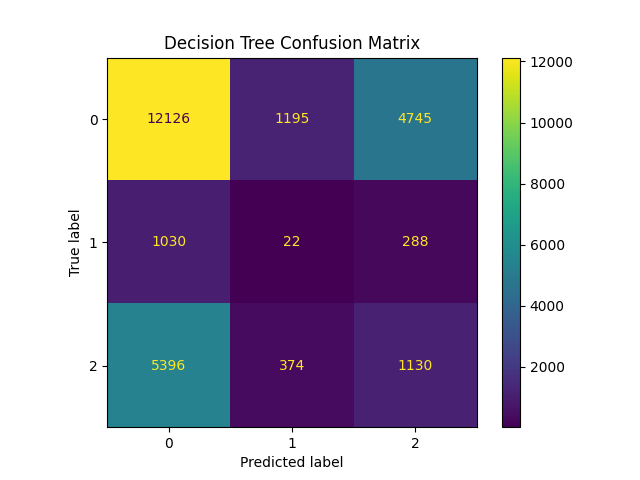
\includegraphics[scale=0.5]{Decision Tree_cm.png}
\centering
\caption{Decision Tree Utilizing Gini Impurity Criterion Confusion Matrix}
\label{fig:dtree}
\end{figure}

\begin{figure}[h!]
    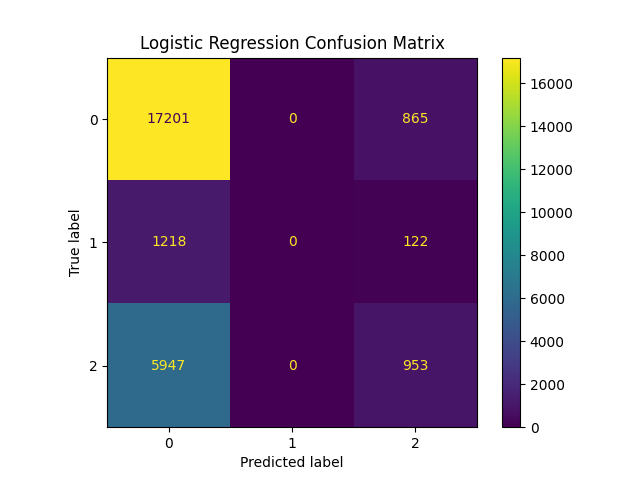
\includegraphics[scale=0.5]{Logistic Regression_cm.png}
    \centering
    \caption{Logistic Regression Utilizing SAGA Solver Confusion Matrix}
    \label{fig:logreg}
    \end{figure}

\begin{figure}[h!]
    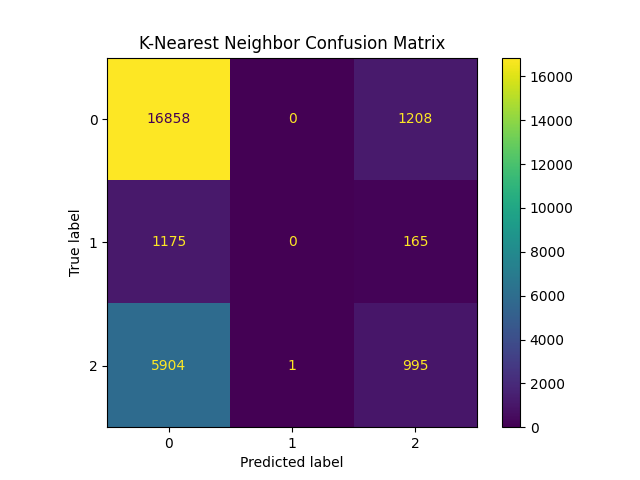
\includegraphics[scale=0.5]{K-Nearest Neighbor_cm.png}
    \centering
    \caption{KNN, K=25 Utilizing Euclidean Metric Confusion Matrix}
    \label{fig:knn}
    \end{figure}

\begin{figure}[h!]
    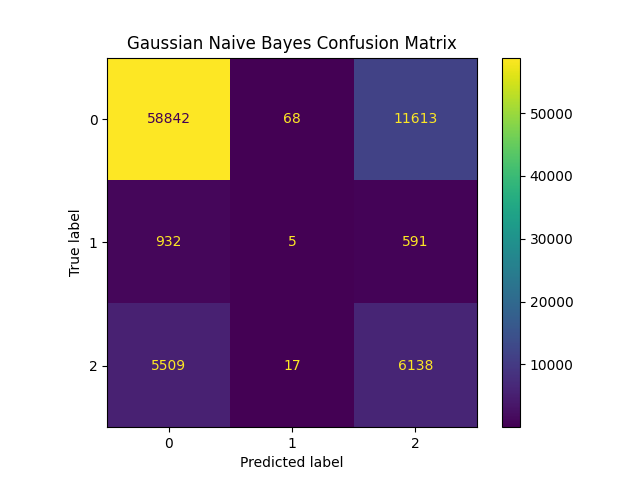
\includegraphics[scale=0.5]{Gaussian Naive Bayes_cm.png}
    \centering
    \caption{Gaussian Naive Bayes Confusion Matrix}
    \label{fig:gaussnb}
    \end{figure}

\clearpage

\begin{figure}[h!]
    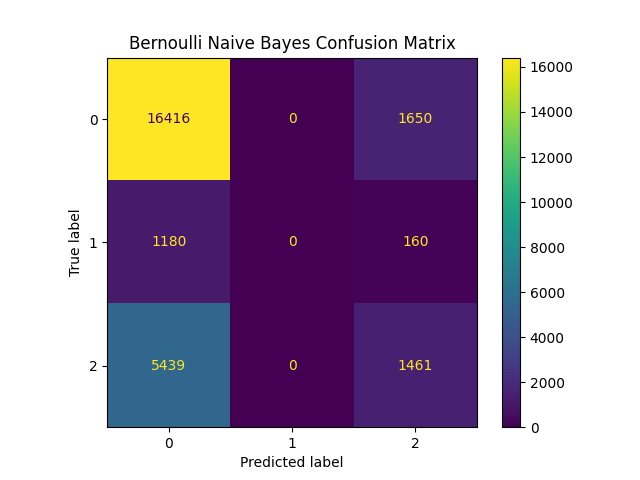
\includegraphics[scale=0.5]{Bernoulli Naive Bayes_cm.png}
    \centering
    \caption{Bernoulli Naive Bayes Confusion Matrix}
    \label{fig:bernnb}
    \end{figure}

\begin{figure}[h!]
    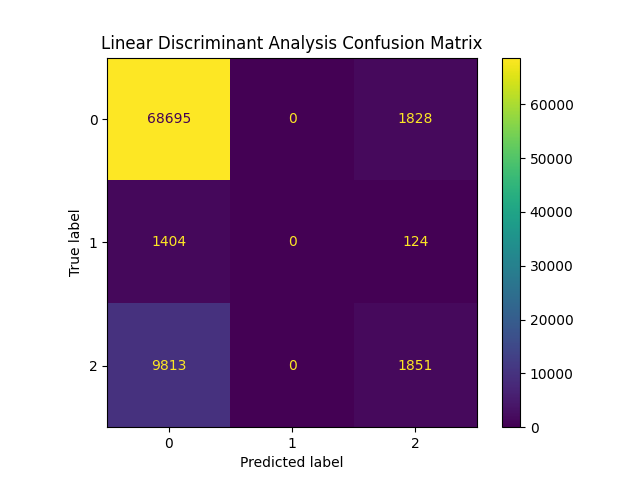
\includegraphics[scale=0.5]{Linear Discriminant Analysis_cm.png}
    \centering
    \caption{LDA Confusion Matrix}
    \label{fig:lda}
    \end{figure}


From these results, the decision tree and Gaussian naïve Bayes are the only models capable to predicting prediabetes, however not very accurately. Objectively, these results are not very good. With the goal of being able to predict an individual's condition early enough for intervention, the low accuracy and precision when classifying prediabetes is concerning.

\subsection{ROC Curves and AUC Rankings}

To further compare the performance of these modes, the receiver operating charactoristics (ROC) curves were plotted for each model and the area under the curve was calculated. The curves specific to classifying diabetes is in Figure \ref{fig:diabetes}, the curves specific to classifying prediabetes is shown in Figure \ref{fig:prediabetes}, and the plots specific to classifying no diabetes in shown in Figure \ref{fig:nodiabetes}.

\pagebreak

\begin{figure}[h!]
    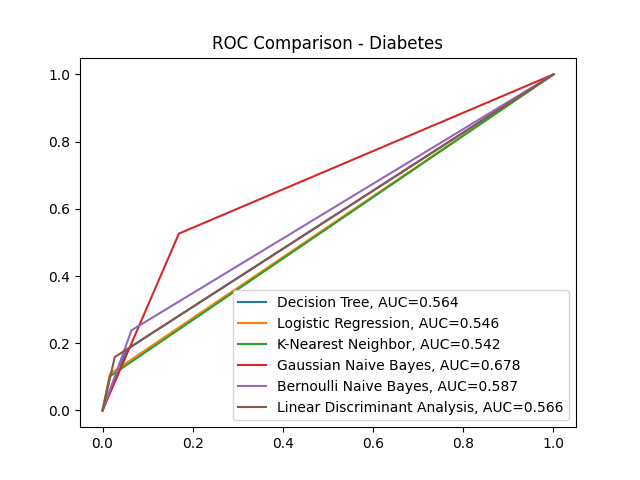
\includegraphics[scale=0.5]{ROC Comparison - Diabetes.png}
    \centering
    \caption{ROC Curves for Diabetes Classification}
    \label{fig:diabetes}
\end{figure}

\begin{figure}[h!]
    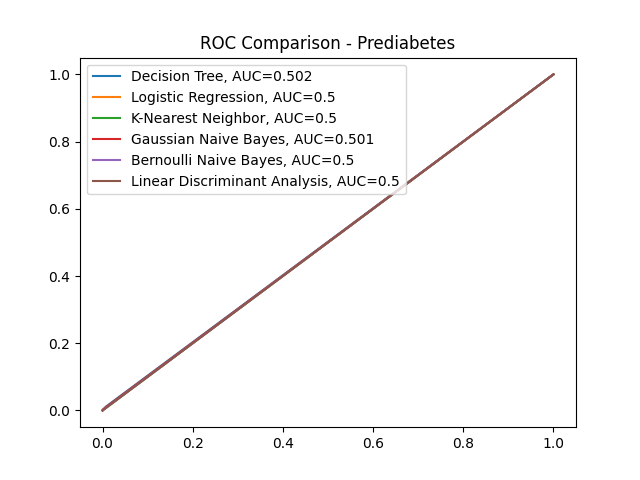
\includegraphics[scale=0.5]{ROC Comparison - Prediabetes.png}
    \centering
    \caption{ROC Curves for Prediabetes Classification}
    \label{fig:prediabetes}
\end{figure}

\begin{figure}[h!]
    \centering
    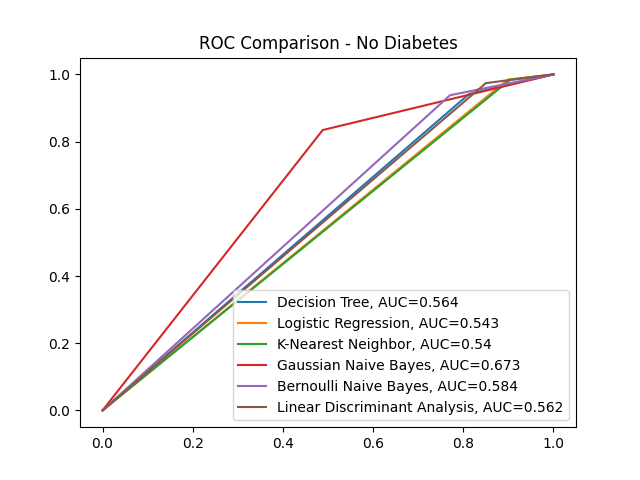
\includegraphics[scale=0.5]{ROC Comparison - No Diabetes.png}
    \label{fig:nodiabetes}
    \caption{ROC Curves for No Diabetes Classification}
\end{figure}

\pagebreak

When ranking the models based on AUC based on each classification, the Gaussian Naïve Bayes proves to be the strongest performing model. All the rankings are shown in Table \ref{table:auc-rankings}.

\begin{table}[h!]
\centering
\begin{tabular}{c | c c c}
Rank & No Diabetes & Prediabetes & Diabetes \\
\hline
1 & Gaussian NB & Decision Tree & Gaussian NB \\
2 & Bernoulli NB & Gaussian NB & Bernoulli NB\\
3 & Decision Tree & - & Decision Tree\\
4 & LDA & - & LDA\\
5 & Logistic Reg. & - & KNN\\
6 & KNN & - & Logistic Reg.\\
\end{tabular}
\caption{Model Rankings Based on AUC}
\label{table:auc-rankings}
\end{table}

\subsection{Cross Validation}

A 10-fold cross validation was performed on each model, both to find the general accuracy of the models and the general precision when classifying prediabetes. The results can be found in Table \ref{table:cross-val} and Table \ref{table:prec-cross-val}. The logistic regression and KNN models were found to be the most accurate with an accuracy of 84.3\%. The model with the lowest accuracy was the Gaussian naïve bayes with an accuracy of 77.5\%. However, the Gaussian naïve Bayes had the greatest precision when predicting prediabetes; its precision rate was 29.9\%. 

\begin{table}[h!]
    \centering
    \begin{tabular}{c | c c }
        Model & Mean Accuracy & Standard Dev. \\
        \hline
        Decision Tree &	0.820 &	0.003 \\
        Logistic Reg. &	0.843 &	0.005 \\
        KNN &	0.843 &	0.001 \\
        Gaussian NB &	0.775 &	0.009 \\
        Bernoulli NB &	0.824 &	0.002 \\
        LDA &	0.841 &	0.005 \\
    \end{tabular}
    \caption{10-Fold Cross Validation Accuracy}
    \label{table:cross-val}
\end{table}

\begin{table}[h!]
    \centering
    \begin{tabular}{c | c c }
        Model & Mean Precision & Standard Dev. \\
        \hline
        Decision Tree &	0.010 &	0.005 \\
        Logistic Reg. & 	0.000 &	0.000 \\
        KNN & 	0.000 &	0.000 \\
        Gaussian NB & 	0.298 &	0.399 \\
        Bernoulli NB & 	0.000 &	0.000 \\
        LDA	 & 0.000 &	0.000 \\
    \end{tabular}
    \caption{10-Fold Cross Validation Precision of Predicting Prediabetes}
    \label{table:prec-cross-val}
\end{table}

\section{Discussion}
\label{sec:discussion}

Overall, the best classification model for this dataset was the Gaussian naïve Bayes classifier. This model was the only model capable of classifying the prediabetes class. However, if this were not the main objective of this investigation, based on these results, the analyst would have to decide what is more important: being able to classify prediabetes or the accuracy of making an overall classification. If the analyst values the capacity to predict prediabetes, the Gaussian naïve Bayes classifier would be the best fit. However, if the analyst values overall accuracy of the classification predictions, the logistic regression, KNN, or LDA models would be better. In general, these recommendations are only based on these models presented in the investigation. The low precision and accuracy may indicate a different model altogether should be examined for this dataset. 

The discrepancy between the precision and accuracy of the predictions was unexpected. This investigation showed that a model's accuracy cannot be the only indicator of performance. Interestingly, the model with the lowest average accuracy was the Gaussian naïve Bayes. However, it showed the greatest precision when making individual classifications. For real-world applications, it is normal to have a high imbalance between classifications within a dataset. In this case, over 80\% of the dataset indicated no diabetes and only 2\% of the dataset made up the prediabetes category. The problem with using accuracy for a dataset with such imbalance is that accuracy treats all classes as equally important \cite{b13}. For this dataset and target classification problem, the precision is a more reliable indicator of performance as it measures how well the model predicts each individual classification. Using precision as the main performance indicator in this scenario is also very important as the cost of false positives is high; the model should therefore minimize false positives. This is crucial in healthcare scenarios (e.g. the classification of diabetes) where accurate identification of individuals at risk is very important.

In the future, addressing the dataset's imbalance would significantly enhance the models' accuracy. Some strategies to alleviate this issue include resampling the data, using a different model that can handle imbalanced datasets more efficiently, and collecting more data in general. If resampling the data, the analyst could either oversample the prediabetes data or undersample the diabetes and no diabetes classes. Other models that can handle imbalanced datasets may be based on boosting or tree-based algorithms \cite{b14}. Another option that could enhance this classification problem is researching the most influential health indicators for diabetes prediction. For example, individuals over the age of 45 are more likely to be afflicted by diabetes \cite{b1}. Using this knowledge, more data can be collected from individuals in this age range, or the dataset could be reduced to only consist of individuals of the age 45 or over. In order to find a better fit model for classifying diabetes and prediabetes, the issue of dataset imbalance must be researched and remedied. 

\begin{thebibliography}{00}
\bibitem{b1}	{“About Prediabetes and Type 2 Diabetes | National Diabetes Prevention Program | CDC.” Accessed: Nov. 23, 2023. [Online]. Available: https://www.cdc.gov/diabetes/prevention/about-prediabetes.html}
\bibitem{b2}	{J. P. Crandall et al., “The prevention of type 2 diabetes,” Nat. Clin. Pract. Endocrinol. Metab., vol. 4, no. 7, pp. 382-393, Jul. 2008, doi: 10.1038/ncpendmet0843.}
\bibitem{b3}	{“Diabetes Health Indicators Dataset.” Accessed: Nov. 23, 2023. [Online]. Available: https://www.kaggle.com/datasets/alexteboul/diabetes-health-indicators-dataset}
\bibitem{b4}	{L. Mueller and R. Hong, “Investigating Decision Trees”.}
\bibitem{b5}	{ArnavR, “Scikit-learn solvers explained,” Medium. Accessed: Nov. 25, 2023. [Online]. Available: https://medium.com/@arnavr/scikit-learn-solvers-explained-780a17bc322d}
\bibitem{b6}	{L. Mueller and R. Hong, “Iris Classification Using Logistic Regression”.}
\bibitem{b7}	{L. Mueller and R. Hong, “Evaluating the Performance of K-Nearest Neighbors Classification”.}
\bibitem{b8}	{S. Ray, “Naive Bayes Classifier Explained: Applications and Practice Problems of Naive Bayes Classifier,” Analytics Vidhya. Accessed: Nov. 25, 2023. [Online]. Available: https://www.analyticsvidhya.com/blog/2017/09/naive-bayes-explained/}
\bibitem{b9}	{L. Mueller, “Comparing Classifications Models Against the Naive Bayes Classifier and Linear Discriminant Analysis Model”.}
\bibitem{b10}	{L. Mueller, “Evaluating Classifications Models using Confusion Matrices”.}
\bibitem{b11}	{L. Mueller, “Ranking Classification Models using Receiver Operating Characteristics”.}
\bibitem{b12}	{L. Mueller and R. Hong, “Using K-Fold Cross Validation on Decision Tree and Logistic Regression Models to Classify Iris Species”.}
\bibitem{b13}	{“Accuracy vs. precision vs. recall in machine learning: what's the difference?” Accessed: Nov. 26, 2023. [Online]. Available: https://www.evidentlyai.com/classification-metrics/accuracy-precision-recall}
\bibitem{b14}	{R. Feki, “Imbalanced data: best practices,” Medium. Accessed: Nov. 26, 2023. [Online]. Available: https://rihab-feki.medium.com/imbalanced-data-best-practices-f3b6d0999f38}



\end{thebibliography}

\end{document}